\documentclass[a4paper, 12pt]{report}


\usepackage[utf8]{inputenc}
\usepackage[T1]{fontenc}
\usepackage[spanish]{babel} 
\usepackage{graphicx}
\usepackage{amsmath}
\usepackage{amssymb}
\usepackage{mathtools}
\usepackage{amsthm}
\usepackage{bbm}
%\usepackage[shortlabels]{enumitem}
\usepackage{enumerate}
\usepackage{array,tabularx}
\usepackage{float}
\usepackage{wrapfig}
\usepackage[export]{adjustbox}
\usepackage[rightcaption]{sidecap}
\usepackage{multirow}
\usepackage{subfig}
\usepackage{capt-of}
\usepackage{captdef}
\usepackage{color}
\usepackage{ebproof}
\usepackage{soul}
\usepackage{hyperref}
\usepackage{stmaryrd}
\usepackage{fullpage}
\usepackage{xcolor}
\usepackage{listings}

\newcommand{\Ra}{\Rightarrow}
\newcommand{\ra}{\rightarrow}
\newcommand{\N}{\mathbb{N}}
\newcommand{\R}{\mathbb{R}}
\newcommand{\te}{\text}
\newcommand{\Lra}{\Leftrightarrow}
\newcommand{\lra}{\leftrightarrow}

\begin{document}

\centerline{\Huge\bf Apuntes de Introducción a la Computación}



\tableofcontents

\chapter{Introducción}

 En este curso planteo a grandes rasgos tres objetivos. El primero es que aprendan las bases de la programación. 
Otro objetivo es que desarrollen la capacidad de utilizar las computadoras con fines matemáticos, como por ejemplo para determinar si un número es primo, o aproximar numéricamente el valor de una integral, o generar gráficas de distintos tipos.
El otro objetivo es que desarrollen la capacidad de entender la computación como un concepto abstracto matemático, para desarrollar programas en base a razonamiento matemático y además poder demostrar matemáticamente propiedades sobre estos programas.
De modo sintético, este curso se trata de programación, de computación para matemática y de matemática para computación.

En este capítulo el objetivo principal es dar una idea básica de qué es la computación, cómo funcionan las computadoras y qué son los lenguajes de programación.



\section{Conceptos básicos de computación e intuiciones}

La computación se trata de operaciones definidas por reglas precisas que operan con objetos finitos y en una cantidad finita de pasos llegan a un resultado.

Los objetos finitos, a los que en general llamaremos {\bf datos}, pueden ser por ejemplo números naturales, palabras o listas finitas. Cabe aclarar que al decir que los números naturales son finitos nos referimos a que cada número natural es un objeto finito. Por supuesto que el conjunto de todos los números naturales, por otra parte, es infinito.

A una operación definida por reglas precisas que opera con datos y termina en finitos pasos le llamaremos {\bf algoritmo}. Un programa es lo mismo que un algoritmo. Un ejemplo de algoritmo es el de la suma que se aprende en la escuela. Dados dos números, aplicando una secuencia finita de pasos bien definida se llega al resultado.


Una buena analogía consta de las recetas de cocina. Sin embargo, hay una diferencia importante. En las recetas de cocina, por la naturaleza de la situación, pueden haber ciertas ambigüedades, o puntos en los que hay que tomar una decisión, de modo que si dos personas realizan la misma receta el resultado puede ser distinto, sin que ninguno de los dos lo haya hecho mal. Pueden haber frases como <<un poquito de sal>> que según la persona se traduzcan a distintas cantidades. En computación, un algoritmo bien ejecutado debe tener un único resultado correcto, como ocurre con la suma. Que las reglas sean precisas significa que no hay margen de variabilidad en lo que se debe hacer, ni puntos en los que un ser con voluntad propia deba pensar y tomar una decisión. Esto es importante por dos motivos. Primero, asegura que si se realiza por una persona, hay un único resultado correcto. Segundo (y tal vez más importante), es necesario para que pueda ser realizado automáticamente por una computadora, que en lugar de un ser con pensamiento y voluntad es una cosa.

Como los algoritmos deben estar bien definidos y no puede haber ninguna ambigüedad, son en esencia conceptos matemáticos. De hecho, la computación teórica es una rama de la matemática.
\subsection{Bases de la formalización matemática}

Una forma de representar algoritmos en computación teórica es mediante funciones $f:\N\to\N$, donde la idea es que si $n$ es la entrada del programa, entonces $f(n)$ es la salida. Como se trata de un algoritmo, no puede ser cualquier función, sino una que puede calcularse en finitos pasos con reglas precisas. A primera vista puede parecer que usar solamente números naturales es una restricción, pero de hecho alcanza para hablar de todo lo que se puede programar. De hecho, dentro de la computadora todos los distintos tipos de datos  se representan con secuencias de bits (\emph{binary digits}, es decir dígitos binarios: 0 o 1) y cualquier secuencia de bits se puede interpretar también como un número escrito en binario. Por lo tanto, todos los datos finitos se pueden representar con números (en general muy grandes). Debido a esto, un programa que recibe como entrada una imagen y retorna la imagen con alguna modificación, por ejemplo, se puede ver como una función $f:\N\to\N$ que recibe el número que codifica la imagen original y retorna el número que codifica la imagen modificada.

Hay distintos formalismos que permiten definir funciones $f:\N\to\N$ computables, es decir, que corresponden a algoritmos. Algunos de ellos son las máquinas de Turing, el cálculo lambda y la teoría de las funciones recursivas. Notablemente, aunque todos son formalismos muy distintos, siempre dan lugar a exactamente el mismo conjunto de funciones computables. Este conjunto de funciones computables no es todo $\N^\N$. De hecho, el conjunto de las funciones computables es numerable, por lo que la mayoría de las funciones no lo son.

Por último, está la pregunta de si la definición matemática de función computable corresponde con las funciones que en el mundo físico se pueden calcular con una computadora. La Tesis de Church-Turing conjetura que efectivamente es el caso. Al ser algo del mundo físico y salirse de la matemática, no hay ninguna prueba formal, pero en general es asumido como cierto.


\section{Arquitectura de Von Neumann}\label{sec-ArqVonNeu}

La arquitectura de Von Neumann es un modelo para computadoras físicas, a diferencia de formalismos como las máquinas de Turing, que son conceptos puramente teóricos.

Primero sería bueno decidir qué consideramos como una computadora. Digamos que es un dispositivo físico que puede automáticamente calcular funciones computables y que tiene mecanismos para interactuar con el entorno. Podemos pensar que es una caja negra que de alguna forma calcula funciones computables y además tiene algún mecanismo por el cual podemos ingresar información (por ejemplo con un teclado) y algún mecanismo por el cual puede devolver información (por ejemplo con una pantalla).

La arquitectura de Von Neumann define que la computadora tiene tres componentes principales que interactúan entre sí: un {\bf procesador }(CPU), una {\bf memoria} y un subsistema de {\bf entrada y salida} (figura \ref{fig-ArqVN}). A la conexión entre las distintas componentes se le llama {\bf bus}. El procesador es un dispositivo con la capacidad de ejecutar un conjunto finito de operaciones básicas, llamadas  instrucciones. La idea es que un programa está dado por una secuencia finita de instrucciones. Si bien las instrucciones son finitas (y en general bastante sencillas), al usarlas de forma secuencial se puede implementar cualquier función computable. Tanto la secuencia de instrucciones que conforma un programa como los datos con los que este opera se guardan en la memoria. El subsistema de entrada y salida permite que la computadora interactúe con el entorno (por ejemplo con un usuario que ingresa datos y observa resultados o con otra computadora dentro de una red).

Todas las componentes de la computadora se construyen con circuitos electrónicos y usando la abstracción del {\sl bit}, que significa dígito binario, es decir {\tt 0} o {\tt 1}. Claramente el bit es un concepto abstracto que no existe de por sí en los circuitos eléctricos. Lo que se hace es tomar una convención, como que si circula corriente significa 1 y si no significa 0, o que cierto voltaje significa 1 y cierto voltaje significa 0. Sea cual sea la convención, lo importante es que se pueden construir circuitos con entrada y salida que implementen cualquier operación finita. Por ejemplo, se puede armar un circuito con 4 bits de entrada, $a_0,a_1,b_0,b_1$ y tres bits de salida $c_0,c_1,c_2$ tal que si tomamos la entrada como la codificación en binario de dos números entre $0$ y $3$, la salida sea la codificación en binario de la suma. En general, para cada función $f:\{0,1\}^n\to\{0,1\}^m$ se puede construir un circuito con $n$ bits de entrada y $m$ bits de salida que implementa la función~$f$. A estos se les llama {\sl circuitos combinatorios}. Junto con otro tipo de circuitos llamados {\sl secuenciales} (que funcionan por etapas y además de la entrada actual dependen de las entradas anteriores, o de un estado que puede ir variando), son un elemento base de las computadoras, tal vez el principal.




\begin{figure}
	\centering
	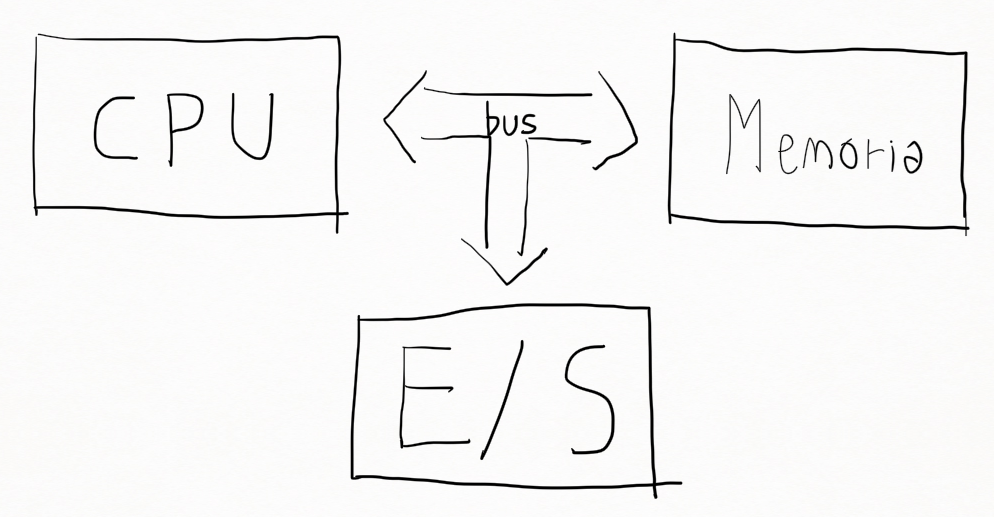
\includegraphics[scale=0.3]{ArqVN.png}
	\caption{Esquema de los componentes de la arquitectura de Von Neumann.}
	\label{fig-ArqVN}
\end{figure}

El procesador tiene tres componentes que cumplen distintas funciones: la unidad de control, la unidad aritmética lógica (ALU) y el banco de registros. La unidad aritmética lógica consta de varios circuitos combinatorios que implementan operaciones básicas, como por ejemplo operaciones lógicas como <<y>>, <<o>> y <<no>>, operaciones aritméticas como suma y multiplicación (para números codificado con una cantidad fija de bits) u operaciones básicas sobre cadenas e bits, como el {\sl shift}, que traslada cada bit un lugar a la derecha o la izquierda. El banco de registros consta de ciertos registros (un tipo de circuito que almacena valores) en general variables que se usan para el funcionamiento de la CPU. Por ejemplo, pueden tener los argumentos de las operaciones que va a realizar la unidad aritmética lógica. También hay un registro de particular importancia llamado {\sl program counter}, que indica la posición de memoria de la siguiente instrucción a ejecutar (es de suma importancia, ya que la idea del CPU es ejecutar secuencias de instrucciones). Finalmente, la unidad de control es un circuito secuencial que se encarga de llevar a cabo las instrucciones, usando la unidad aritmética lógica y el banco de registros. Estos circuitos secuenciales están hechos para que automáticamente se lea e identifique la instrucción que indica el program counter, se carguen nuevos datos en los registros (si es necesario), se realice la operación indicada en la ALU y se guarde el resultado donde corresponda (si hay que hacer alguna operación), y que el program counter avance a la siguiente instrucción, para poder repetir el proceso.

Respecto a la suma, la ALU al ser un circuito combinatorio, es en realidad como una tabla que tiene el resultado para cada combinación de operandos. Las sumas que se realizan directamente por la ALU pueden ser por ejemplo de números representados por uno o dos bytes (donde un byte es por definición una secuencia de 8 bits). Como la cantidad de números representables crece exponencialmente con la cantidad de bits, hacer sumas de números más grandes por la ALU (que lo que hace es tener una tabla con todos los resultados) es extremadamente ineficiente. Lo que se hace para realizar sumas con números más grandes es descomponerlas como una secuencia de instrucciones más sencillas. Esto es como lo que se hace en los algoritmos aritméticos básicos. Pensemos por ejemplo en el producto. Está la tabla de multiplicación que uno se aprende de memoria (lo cual es análogo a lo que está en los circuitos de la ALU) pero luego a partir de eso, siguiendo un algoritmo (secuencia de instrucciones) se puede calcular la multiplicación de números de cualquier cantidad de cifras sin precisar saber nada más de memoria.

La memoria es un dispositivo electrónico capaz de almacenar muchos valores, los cuales pueden ser leídos o modificados. Tiene la estructura de un gran vector de bytes, indizado por secuencias de bits de largo fijo. Por ejemplo, si se usan dos bits para indizar, los lugares de la memoria serían el {\tt 00}, el {\tt 01}, el {\tt 10} y el {\tt 11}, cada uno de los cuales contendría un byte de información. En las computadoras actuales la memoria suele tener del orden de $2^{32}$ lugares de memoria, es decir 4GB ($2^{10}$ bytes es un KB, $2^{20}$ es un MB y $2^{30}$ es un GB). Se trata de la llamada memoria RAM. Actualmente la cantidad de bits que se usa para indizar es 64 (la llamada arquitectura de 64 bits), pero eso no implica que todas las palabras que se puedan formar correspondan a direcciones válidas (en computadoras personales no existe actualmente memoria de $2^{64}$ bytes, que serían como 16 mil millones de gigabytes). Conceptualmente el banco de registros del procesador es como una memoria. El motivo de que existan las dos cosas es que el banco de registros es memoria de mejor calidad y más cara que se reserva para estar dentro de la CPU, mientras que la memoria RAM es más lenta pero más económica para tener en grandes cantidades.

\subsection{Ejemplo de programa}

Hagamos un ejemplo del funcionamiento de una computadora. Supongamos que tenemos 8 registros (enumerados) de un byte cada uno y que las direcciones de memoria son indizadas también por un byte. Supongamos que tenemos las siguientes instrucciones
\begin{itemize}
	\item {\tt LOAD}. Instrucción con dos parámetros: {\tt M} y {\tt R}, que lo que hace es cargar en el registro {\tt R} el contenido de la dirección de memoria {\tt M}.
	\item {\tt SAVE}. Instrucción con dos parámetros: {\tt M} y {\tt R}, que lo que hace es guardar en la dirección de memoria {\tt M} el contenido del registro {\tt R}.
	\item {\tt ADD}. Instrucción con tres parámetros: $\mathtt{R_1}$, $\mathtt{R_2}$ y $\mathtt{R_3}$ que lo que hace es sumar el contenido de los registros $\mathtt{R_1}$ y $\mathtt{R_2}$ y guardar el resultado en el registro $\mathtt{R_3}$.
\end{itemize}


Respecto a la operación {\tt ADD}, como los contenidos de los registros son bytes, o sea 8 bits, se considera que cada secuencia de 8 bits representa en binario un número entre $0$ y $2^8-1$. En caso de que el resultado se salga del rango, se le sustraye $2^8$ al resultado (formalmente, es la suma de $\mathbb{Z}_{2^8}$, es decir aritmética modular).

Por otra parte, cada instrucción está codificada por un byte. Supongamos que el código de {\tt LOAD} es {\tt 00000001}, el de {\tt SAVE} es {\tt 00000010} y el de {\tt ADD} es {\tt 00000011}.

Asumamos también que los tres primeros registros, $\mathtt{R_1}$, $\mathtt{R_2}$ y $\mathtt{R_3}$ se identifican con los bytes {\tt 00000001}, {\tt 00000010} y {\tt 00000011}.

Supongamos que queremos un programa que lo que haga es sumar los contenidos de las direcciones de memoria {\tt 10000001} y {\tt 10000010} y guardar el resultado en la dirercción {\tt 10000011}. Podríamos hacerlo realizando cuatro instrucciones. Primero un {\tt LOAD} para cargar el contenido de la primera dirección de memoria en el registro 1, luego otro {\tt LOAD} para cargar el contenido de la segunda dirección de memoria en el registro 2, luego un {\tt ADD} para sumar los contenidos de los registros 1 y 2 y guardar el resultado en el registro 3 y finalmente una {\tt SAVE} para guardar el contenido del registro 3 en la tercera dirección de memoria. Primero escribamos las instrucciones de un modo un poco más abstracto (para no ir de una a los 0s y 1s).  Definamos las direcciones de memoria {\tt 10000001}, {\tt 10000010} y {\tt 10000011} como $\mathtt{M_1}$, $\mathtt{M_2}$ y $\mathtt{M_3}$, respectivamente. El programa sería lo siguiente.
\begin{align*}
	&\mathtt{LOAD} \quad\mathtt{M_1~R_1}\\
	&\mathtt{LOAD}  \quad\mathtt{M_2~R_2}\\
	&\mathtt{ADD}  \quad\mathtt{R_1~R_2~R_3}\\
	&\mathtt{SAVE}  \quad\mathtt{M_3~R_3}
\end{align*} 
Esto último es lo que se considera como un programa escrito en {\sl assembler}. Es una forma de programar en la que cada línea es una instrucción del procesador, pero se pueden usar los nombres de las instrucciones y nombres de lugares de memoria, en lugar de tener que escribir todo en bits. El mismo programa escrito ahora en código máquina, es decir en bits, exactamente como iría en la memoria, sería:
\begin{align*}
	&\mathtt{00000001} \quad\mathtt{10000001~00000001}\\
	&\mathtt{00000001}  \quad\mathtt{10000010~00000010}\\
	&\mathtt{00000011}  \quad\mathtt{00000001~00000010~00000011}\\
	&\mathtt{00000010}  \quad\mathtt{10000011~00000011}
\end{align*}
La organización en líneas del código es para que sea más fácil de leer, pero el programa de hecho es simplemente 0000000110000001000000010000000110000010000000100000001100 0000010000001000000011000000101000001100000011. Si tenemos en alguna parte de la memoria esa secuencia de bytes y el program counter indicando la dirección donde comienza, la computadora automáticamente lo ejecutará. Esto se ilustra en la figura \ref{fig-ArqVNEjProg}.

Cabe resaltar que este es un ejemplo muy sencillo. Hay otros tipos de instrucciones (por ejemplo las que modifican el program counter y permiten realizar ciclos) y los programas suelen ser mucho más largos. De hecho, cuales son exactamente las instrucciones y cómo se codifican varía de un procesador a otro.

\begin{figure}
	\centering
	\includegraphics[scale=0.33]{ArqVNEjProg.png}
	\caption{Esquema de una computadora con un programa.}
	\label{fig-ArqVNEjProg}
\end{figure}

\section{Lenguajes de programación y compiladores}

Dada una computadora que sigue la arquitectura de Von Neumann, se puede implementar cualquier función computable con algún programa escrito en código máquina. Sin embargo, hay algunas características poco prácticas.
\begin{itemize}
	\item Es relativamente difícil escribir programas como secuencias de instrucciones de máquina. En general hay muchos más detalles que entran en juego que en el ejemplo dado y hace falta mucho esfuerzo para escribir programas que hagan operaciones complejas.
	\item Distintos procesadores suelen tener distintas instrucciones. Además, incluso cuando la instrucción es la misma puede estar codificada distinto. Por ejemplo, puede que en un procesador {\tt 00000001} sea el código de la suma y en otro sea el código de la operación de cargar en un registro. Por lo tanto, un programa que se escribe para un procesador probablemente no funcione en otro.
\end{itemize}
Estos factores dificultan escribir programas y hacen que solamente lo puedan hacer especialistas. Sin embargo, con el tiempo se desarrolló un concepto que mejora la situación, haciendo que sea más fácil desarrollar un programa y que la curva de aprendizaje sea más corta. Se trata de los {\bf lenguajes de programación}.

Los lenguajes de programación introducen abstracciones que permiten escribir programas sin preocuparse por detalles técnicos de cómo se resuelve con instrucciones del procesador. Por ejemplo, se introduce el concepto de las variables para trabajar con datos sin preocuparse por en qué direcciones de memoria están ni de cómo se utilizan los registros para operaciones. Por ejemplo, se si tenemos tres variables {\tt x, y} y {\tt z}, para sumar los contenidos de las primeras dos y guardarlo en la tarcera, simplemente habría que escribir:
$$\mathtt{z} = \mathtt{x}+\mathtt{y}
$$
sin preocuparse ni por en qué dirección va cada una ni de si hay que usar registros para realizar la suma o no.

Un programa escrito en un lenguaje de programación es un archivo de texto. Se compone por líneas escritas con caracteres comunes que representan operaciones de forma clara (para una persona). Las instrucciones escritas en un lenguaje de programación no pueden ser ejecutadas directamente por un procesador (estos solo entienden ceros y unos). En este punto entran en juego los {\bf compiladores}. Estos son programas cuya función es traducir un programa escrito en un lenguaje de programación a un programa en código máquina. Se los puede pensar como funciones cuya entrada es un programa escrito en un lenguaje de programación y su salida es una secuencia de instrucciones de procesador (lenguaje máquina) que hace lo mismo. El proceso usual al programar es el siguiente: primero se escribe el programa en un lenguaje de programación, luego se usa un compilador para traducirlo a código de máquina y finalmente se lo ejecuta.

Los lenguajes de programación junto con los compiladores solucionan las dos desventajas previamente mencionadas. Por una parte, escribir en un lenguaje de programación es más fácil que en lenguaje máquina. Por otra parte, un lenguaje de programación suele tener compiladores para distintos procesadores, de modo que un mismo programa escrito en este lenguaje puede ser compilado a código máquina de distintos procesadores y por lo tanto ser ejecutado en cada uno de ellos.

Se dice que un lenguaje de programación es de alto o bajo nivel según el nivel de abstracción que hay por sobre el lenguaje de máquina (instrucciones del procesador). Escribir directamente las instrucciones del procesador o código en assembler es de bajo nivel, mientras que usar un lenguaje de programación que incluye abstracciones como variables, estructuras de datos o iteraciones es de alto nivel. Entre los distintos lenguajes de programación hay varios niveles de abstracción.


El lenguaje {\tt c} (así como {\tt pascal}) es un lenguaje de relativamente bajo nivel, pues tiene abstracciones como las previamente mencionadas, pero no está {\sl tan} lejos del lenguaje máquina. Mirando un programa escrito en {\tt c}, para alguien con experiencia no es tan difícil darse cuenta de cómo podrían ser las instrucciones en lenguaje máquina.

Por otra parte, el lenguaje {\tt python}, que es el que usaremos en el curso, es de muy alto nivel. Esto significa que tiene abstracciones muy complejas por sobre el lenguaje máquina, las cuales hacen que se pueda programar en base a razonamientos intuitivos sin saber cómo se haría en lenguaje de máquina. De hecho puede ocurrir que una sola línea de código en {\tt python} corresponda a cientos de instrucciones del procesador, con lo que se resuelven automáticamente detalles técnicos y se le ahorra trabajo al programador. En general usar un lenguaje de programación de alto nivel es más fácil que usar uno de bajo nivel. La desventaja que tienen es que las abstracciones pueden hacer que el programa no sea lo más eficiente posible. En general un programa escrito en {\tt c} es mucho más rápido que uno equivalente en {\tt python} (pero mucho más difícil de escribir).

\chapter{Programación en python}

En este capítulo se presentan los conceptos básicos para programar en el lenguaje python. Si bien se trata de un lenguaje específico, los conceptos se aplican de forma muy similar en otros. El objetivo de este material es presentar los elementos de forma conceptual. Para asimilarlos bien se recomienda complementar con otros materiales que incluyan más ejemplos y además escribir y ejecutar código uno mismo (para instalación y ejecución ver sección \ref{sec-instalyEjec}).

Respecto a materiales que incluyen ejemplos, se recomienda el tutorial de la documentación oficial de python: \href{https://docs.python.org/es/3.13/tutorial/index.html}{https://docs.python.org/es/3.13/tutorial/index.html}. Ese tutorial contiene mucho más que lo que se necesita para el curso. Se recomienda ver todo el capítulo 3 y algunos conceptos del 4 para ver ejemplos, pero sin preocuparse por detalles técnicos (hay explicaciones pensadas para gente que ya conoce conceptos de programación por otros lenguajes).

Cabe aclarar que lo que se ve en este curso es solo una pequeña introducción a python.

\section{Instalación y ejecución}\label{sec-instalyEjec}

Instalar python es principalmente instalar el compilador que traduce el código en python a lenguaje máquina, de modo que podamos ejecutar lo que programemos. Un detalle técnico es que en lugar de llamársele <<compilador>> se le llama <<intérprete>>. Esto es porque en lugar de pasar todo el programa a lenguaje máquina y luego ejecutarlo, va pasando las líneas de código a lenguaje máquina una por una a la vez que se van ejecutando. Se dice que es un compilador cuando primero se traduce todo a lenguaje máquina y luego se lo ejecuta.

En el sistema operativo linux, en general python ya viene instalado por defecto. Por otra parte, en windows no es el caso (nos enfocaremos en este sistema operativo, ya que quienes utilizan linux es más probable que ya sepan ejecutar python). Una forma de instalarlo es descargando el instalador desde el sitio web de python y ejecutándolo (\href{https://www.python.org/downloads/}{https://www.python.org/downloads/}). Durante la instalación es importante marcar la opción de <<Add python.exe to PATH>> (figura \ref{fig-InstallPython}), por motivos que vermos a contiuación.

\begin{figure}
	\centering
	\includegraphics[scale=0.5]{InstallPython.png}
	\caption{Es importante marcar la opción <<Add python.exe to PATH>>.}
	\label{fig-InstallPython}
\end{figure}

Vamos a ejecutar python desde una ventana de comandos (o terminal). Esto es una ventana a través de la cual se le escriben comandos al sistema operativo. En windows se llama Windows PowerShell o símbolo del sistema.

Si la instalación de python es correcta, al abrir una ventana de comandos, si se escribe python y se toca enter, comienza a ejecutarse el intérprete, el cual nos permite ir ingresando instrucciones una a una. Los tres símbolos de >~significan que el intérprete está listo para recibir instrucciones. Una primera cosa que se puede hacer es usarlo como calculadora, escribiendo expresiones aritméticas y tocando enter (figura \ref{fig-cmdPython}).

Al escribir python, lo que se hace es ejecutar el intérprete. Para que esto funcione, el sistema operativo debe tener la dirección en la que python está instalado dentro de una cierta lista. Esto es lo que se hace al marcar la opción <<Add python.exe to PATH>> durante la instlación. Luego de haber ejecutado python en la ventana de comandos, el uso del intérprete ocurre dentro de esta misma ventana, sin usarse ninguna interfaz gráfica (a diferencia de la mayoría de los programas que utilizamos). En general no hay necesidad de nada más sofisticado.

\begin{figure}
	\centering
	\includegraphics[scale=0.5]{cmdPython.png}
	\caption{Ventana de comandos con el intérprete de python.}
	\label{fig-cmdPython}
\end{figure}

Con la modalidad de uso del intérprete que vimos, se escriben y ejecutan lineas una a una. Por otra parte, se puede escribir un archivo con varias lineas de código y pasárselo al intérprete para que lo ejecute. El código se escribe en un archivo de formato <<.py>>. Para escribir este tipo de archivos se puede usar cualquier editor de texto, pero se recomienda utilizar un editor de código especializado. Uno muy popular actualmente es visual studio code (\href{https://code.visualstudio.com/}{https://code.visualstudio.com/}). Una vez que se escribió el archivo con el código y se lo tiene guardado en una carpeta, hay que abrir una ventana de comandos en esa carpeta (cada ventana de comandos trabaja en alguna carpeta particular) e ingresar <<python>> seguido del nombre del archivo con el <<.py>> incluido. Esto se ejemplifica en la figura \ref{fig-ejecPython}.

Para todo lo que mencionamos en esta sección, buscando en internet (motores de búsqueda como google, o sitios con contenido audiovisual como youtube) se encuentran muchos tutoriales. 

\begin{figure}
	\centering
	\includegraphics[scale=0.4]{ejecPython.png}
	\caption{A la izquierda visual studio code con el código del archivo llamado programa.py. Al centro se ve la carpeta llamada ejemplo en la que está el archivo. Dentro de esa carpeta se abre la terminal. A la derecha se ve la terminal en la que se escrie <<python programa.py>>. Antes del símbolo >, a la izquierda de <<python>>, se indica la carpeta en la que está la terminal.}
	\label{fig-ejecPython}
\end{figure}
\section{Tipos de datos}

Una de las abstracciones que aportan los lenguajes de programación consiste en los tipos de datos. Se trata de la abstracción de distintos tipos de objetos, como enteros, texto o listas, cada uno de los cuales tiene distintos posibles valores y distintas operaciones que se pueden aplicar. Por supuesto que todos estos objetos se codifican como secuencias de bits, pero poder trabajar pensando en términos de objetos de distinto tipo hace que programar sea más intuitivo. Veamos algunos de los tipos de datos que tiene python.

\subsection{Booleanos}

Los booleanos conforman un tipo de datos que representa valores de verdad. Tiene solo dos objetos: {\tt True} y {\tt False}. Se tienen las operaciones booleanas básicas: {\tt not}, {\tt and} y {\tt or}. Hay algunos ejemplos en la figura \ref{fig-ejemploBool}. En general los booleanos por sí solos no suelen ser de mucha utilidad. Su principal aplicación es en condicionales e iteraciones, que estudiaremos en lo siguiente.

\begin{figure}
	\centering
	\includegraphics[scale=0.6]{ejemploBool.png}
	\caption{Ejemplos de operaciones con booleanos.}
	\label{fig-ejemploBool}
\end{figure}

\subsection{Enteros}

Se trata de un tipo de datos para representar enteros naturales. Los objetos son {\tt 0}, {\tt 1} {\tt -1}, {\tt 2}, {\tt -2}, etc. Tienen las operaciones aritméticas elementales, que se muestran en la figura \ref{fig-ejemploInt}. Notar que la división entera es con dos barras. Una barra sola es otra operación que veremos en la brevedad. Por otra parte se tienen las operaciones de comparación, que reciben dos enteros y retornan un booleano. Se muestran en la figura \ref{fig-ejemploComp}. En el caso de la igualdad, si se escribe un solo símbolo <<=>> es una asignación, lo cual veremos más adelante.

\begin{figure}
	\centering
	\includegraphics[scale=0.6]{ejemploInt.png}
	\caption{Operaciones aritméticas básicas. Lo que está escrito después de los \# son comentarios. Los comentarios son ignorados por el intérprete, la función que cumplen es de aclaraciones para personas que lo leen.}
	\label{fig-ejemploInt}
\end{figure}

\begin{figure}
	\centering
	\includegraphics[scale=0.6]{ejemploComp.png}
	\caption{Comparaciones entre enteros. }
	\label{fig-ejemploComp}
\end{figure}

\subsection{Números de punto flotante}

Se trata de una representación para operar con números reales usando información finita. De hecho lo que representan es un conjunto finito de números racionales, pero a menos de cierta aproximación se opera con ellos igual que con números reales. Estos números se escriben con la notación usual para números con parte fraccionaria o con notación científica, en ambos casos separando la parte fraccionaria con un punto. Están las mismas operaciones aritméticas y comparaciones, salvo por la división. Con punto flotante no se pueden usar // ni \%. En su lugar se usa un único / para la división de números reales. Un detalle importante es que si aplicamos la operación / a enteros, el resultado es de punto flotante, independientemente de que la división de exacta o no. Se presentan ejemplos en la figura \ref{fig-ejemploFloat}.

Los números de punto flotante tienen limitaciones debido al hecho de que se pueden representar solo finitos números. Por ejemplo, si a {\tt 1.0} le sumamos un número muy chico, se redondea a {\tt 1.0}, lo cual puede ser problemático en algunas situaciones. Ignoraremos este problema, pero es un tema relevante dentro del área de análisis numérico.

Hay más operaciones sobre punto flotante que se pueden realizar si importamos la biblioteca {\tt math}. Más adelante en el curso nos centraremos más en las bibliotecas, pero por ahora alcanza con saber que es algo que permite extender el lenguaje con más operaciones. Para incluir el contenido de la biblioteca {\tt math} hay que escribir la instrucción {\tt import math}. Después de eso se pueden utilizar las operaciones incluidas en esta biblioteca. Esto se hace escribiendo el nombre de la biblioteca, un punto y el nombre de la operación. Por ejemplo, tiene una operación de raiz cuadrada que se utiliza escribiendo {\tt math.sqrt()}, donde al argumento lo ponemos entre los paréntesis. Por otra parte, está la operación {\tt math.floor()} que retorna el entero más cercano a la izquierda. Esta última función retorna efectivamente un objeto de tipo entero y no un objeto de tipo punto flotante con valor entero. Se presentan ejemplos en la figura \ref{fig-ejemploMath}.

Se pueden realizar la mayoría de las operaciones aritméticas entre enteros y números de punto flotante. En ese caso, el resultado es de punto flotante.

\begin{figure}
	\centering
	\includegraphics[scale=0.6]{ejemploFloat.png}
	\caption{Ejemplos de números de punto flotante.}
	\label{fig-ejemploFloat}
\end{figure}

\begin{figure}
	\centering
	\includegraphics[scale=0.6]{ejemploMath.png}
	\caption{Ejemplos de operaciones de la biblioteca math.}
	\label{fig-ejemploMath}
\end{figure}


\subsection{Texto}

En python se puede representar texto. Esto se hace encerrándolo entre comillas simples o dobles. En general se les llama strings. Algunos ejemplos son ``Hola.'', ``345'' y ``''. No hay que confundir al string ``345'' con el entero {\tt 345}, pues el primero es simplemente una secuencia de caracteres. Con el símbolo + se puede concatenar caracteres.

\subsection{Listas}

Las listas conforman un tipo de datos compuesto. Cada lista es, como su nombre sugiere, una lista de objetos. Una lista se comienza y se termina con <<[>> y <<]>>. Los distintos elementos se separan con comas. Por ejemplo: {\tt[0,1,4]}, {\tt[``aa'',``a'',``'']}, {\tt [3.5, ``a'']} y {\tt[]}. Las listas pueden tener cualquier cantidad de elementos (a partir de cero) y estos elementos pueden ser de cualquier tipo, incluso otras listas. Por ejemplo {\tt [[],[]]} es una lista con dos elementos, que los dos son la lista vacía. Con + se puede concatenar listas, de modo que {\tt [[],[]] + [1]} es {\tt [[],[],1]}.


\section{Variables y asignaciones}

Las variables son abstracciones que consisten en un lugar de memoria al que se le asigna un nombre, dentro del cual se pueden guardar distintos valores. Nombres válidos de variable son secuencias de caracteres alfanuméricos y <<\_>> en los que el primer carácter no es un número, como por ejemplo {\tt x, x1, total} y {\tt altura\_caja}. Los valores pueden ser de cualquier tipo de dato.

La asignación es la instrucción básicas de python para dar un nuevo valor a una variable. La sintaxis es:
$$\mathtt{var}~=~\mathtt{expr}$$
donde $\mathtt{var}$ es el nombre de la variable al que queremos asignar el valor y $\mathtt{expr}$ es una expresión que calcula el valor a asignar.  Es distinto al uso que se le da al símbolo <<$=$>> en matemáticas, asemejándose más al de <<$:=$>>. La expresión puede ser un objeto fijo, otra variable o algo más elaborado, por ejemplo con operaciones. Incluso puede contener la misma variable {\tt var}. En ese caso para evaluar la la expresión se usa el valor actual de la variable y luego se le asigna el resultado. Si en la expresión ponemos alguna variable aún no definida, se produce un error. Los siguientes son algunos ejemplos.

\begin{verbatim}
>>> x = 10
>>> x #Mostrar el valor de la variable x
10
>>> x = 10 #asignamos el valor 10 a la variable x
>>> x #Mostrar el valor actual de la variable x
10
>>> x*2
20
>>> x1 = x**2
>>> x1
100
>>> x = x + 1
>>> x
11
>>> z = 20
>>> z = z + x2 #Usamos una variable x2 que no definimos antes. Da error
Traceback (most recent call last):
File "<stdin>", line 1, in <module>
NameError: name 'x2' is not defined. Did you mean: 'x'?
>>> lista1 = ["a","b","c"]
>>> lista2 = [1,2,3]
>>> lista3 = lista1 + lista2
>>> lista3
['a', 'b', 'c', 1, 2, 3]
\end{verbatim}
\section{Indizado y slicing}

El indizado se trata de cómo acceder a elementos de ciertos lugares en estructuras de datos compuestas. Vamos a introducirlo para listas y strings (aunque pensando los strings como listas de caracteres es muy análogo).

Dada una variable {\tt x} que tiene una lista y un entero $n$ (o una variable que contiene al entero $n$), tenemos que {\tt x[$n$]} es el elemento número $n$ de la lista. En caso de que {\tt x} contenga un string, es el carácter número~$n$. En python (así como en la mayoría de los lenguajes de programación) la enumeración comienza en 0. Por lo tanto, dada una lista {\tt x}, su primer elemento es {\tt x[0]}. Lo mismo se puede aplicar con strings, caso en el que se retorna un substring formado solamente por el caracter del lugar $n$.

Tanto para listas como para strings, si el índice se pasa del último elemento, se produce un error. En python se puede usar la función {\tt len()} para determinar el largo de una lista o un string. Los índices válidos de {\tt x} van desde {\tt 0} hasta {\tt len(x)-1}.

Por otra parte, el {\sl slicing} consiste en indizar por rangos, obteniéndose sublistas o substrings. La versión más sencilla, dada una lista {\tt x} y dos enteros $n,m$, es {\tt x[$n:m$]}, que resulta en la sublista de todos los elementos con índice $i$ tal que $n\leq i < m$. Notar que el extremo de abajo usa orden inclusivo y el de arriba estricto. En este caso no hay problemas si nos pasamos del último elemento. En todo caso puede quedar la lista vacía o el string vacío.

También se pueden hacer asignaciones a elementos de cierto íncide, permitiendo modificar el valor de cierto lugar de una lista. Con strings no se permite hacer esto.

Veamos ejemplos de todo lo anterior.
\begin{verbatim}
>>> x = [1,2,3,4,5]
>>> s = "Hola 1."
>>> x[0]
1
>>> s[1]
'o'
>>> s[4] #Va a retornar un espacio
' '
>>> len(s)
7
>>> s[6]
'.'
>>> s[7]
Traceback (most recent call last):
File "<stdin>", line 1, in <module>
IndexError: string index out of range
>>> x[5]
Traceback (most recent call last):
File "<stdin>", line 1, in <module>
IndexError: list index out of range
>>> x[0:2]
[1, 2]
>>> x[2:5]
[3, 4, 5]
>>> x[2:10]
[3, 4, 5]
>>> x[6:10]
[]
>>> x[1]=40
>>> x
[1, 40, 3, 4, 5]
\end{verbatim}


\section{Instrucciones}

\section{Condicionales}

\section{Iteraciones}

\section{Procedimientos y funciones}


\end{document}


